%FRACTIONS ON A NUMBER LINE - WORKSHEET 0 (IN-CLASS INSTRUCTION)
\documentclass[12pt, letterpaper, fleqn]{article}

% ----------------------------------------------------------
% PACKAGES
% ----------------------------------------------------------
\usepackage{graphicx}
\usepackage{xcolor}
\usepackage[most]{tcolorbox}
\usepackage{amsmath, amssymb}
\usepackage{fancyhdr}
\usepackage[utf8]{inputenc}
\usepackage[T1]{fontenc}
\usepackage{enumitem}
\usepackage{geometry}
\usepackage{tikz}
\usepackage{needspace}
\usepackage{multicol}

\usetikzlibrary{arrows.meta, calc, shapes.geometric}

% ----------------------------------------------------------
% PAGE SETUP
% ----------------------------------------------------------
\usepackage{times}
\geometry{letterpaper, top=1.25in, bottom=1.25in, marginpar=0.5in}

% ----------------------------------------------------------
% HEADER / FOOTER
% ----------------------------------------------------------
\newcommand{\logowidth}{3cm}
\setlength{\headheight}{20pt}
\setlength{\footskip}{40pt}

\pagestyle{fancy}
\fancyhf{}
\fancyhead[C]{\small\bfseries Fractions on a Number Line}
\fancyfoot[L]{\raisebox{2pt}{
\includegraphics[width=\logowidth]{../kss.png}}}
\fancyfoot[C]{\thepage}
\fancyfoot[R]{3.15.0}

\renewcommand{\footrulewidth}{0.2pt}

% ----------------------------------------------------------
% THEME COLOR
% ----------------------------------------------------------
\definecolor{customteal}{HTML}{2fbdb9}

% ----------------------------------------------------------
% HELPER MACROS
% ----------------------------------------------------------
\newcommand{\blank}{\underline{\hspace{2.2cm}}}
\newcommand{\blanklong}{\underline{\hspace{6.5cm}}}
\newcommand{\blankshorter}{\underline{\hspace{1.5cm}}}

% ----------------------------------------------------------
% DOCUMENT
% ----------------------------------------------------------
\begin{document}

\textbf{Name:} \underline{\hspace{5cm}}
\hfill
\textbf{Date:} \underline{\hspace{3cm}}\\

\begin{tcolorbox}[colback=customteal!20]
    \large\textcolor{black}{\textbf{Fractions on a Number Line}}
\end{tcolorbox}

\vspace{3mm}
\noindent
We can show fractions as points on a number line between 0 and 1.
\begin{center}
\begin{tikzpicture}[scale=1.2]
\draw[latex-latex, thick] (-0.5,0) -- (4.5,0);
\draw[thick] (0,0.15) -- (0,-0.15) node[below] {0};
\draw[thick] (1,0.1) -- (1,-0.1) node[below] {$\frac{1}{4}$};
\draw[thick] (2,0.1) -- (2,-0.1) node[below] {$\frac{2}{4}$};
\draw[thick] (3,0.1) -- (3,-0.1) node[below] {$\frac{3}{4}$};
\draw[thick] (4,0.15) -- (4,-0.15) node[below] {1 (or $\frac{4}{4}$)};
\filldraw[red] (3,0) circle(2pt);
\end{tikzpicture}
\end{center}
The red dot is located at $\dfrac{3}{4}$.

\newpage
\begin{tcolorbox}[colback=customteal!20]
    \large\textcolor{black}{\textbf{Guided Practice}}
\end{tcolorbox}

\vspace{5mm}
\noindent
Write the fraction for the letter plotted on each number line.

\vspace{8mm}
\begin{enumerate}[itemsep=4.5cm, leftmargin=0.6cm]
\item 
\begin{tikzpicture}[scale=1.2]
\draw[latex-latex, thick] (-0.5,0) -- (3.5,0);
\draw[thick] (0,0.15) -- (0,-0.15) node[below] {0};
\draw[thick] (1,0.1) -- (1,-0.1);
\draw[thick] (2,0.1) -- (2,-0.1);
\draw[thick] (3,0.15) -- (3,-0.15) node[below] {1};
\filldraw[blue] (2,0) circle(2.5pt) node[above] {A};
\end{tikzpicture}
\\
Letter A represents: \blank

\item 
\begin{tikzpicture}[scale=1.2]
\draw[latex-latex, thick] (-0.5,0) -- (6.5,0);
\draw[thick] (0,0.15) -- (0,-0.15) node[below] {0};
\draw[thick] (6,0.15) -- (6,-0.15) node[below] {1};
\foreach \x in {1,2,3,4,5} {
  \draw[thick] (\x, 0.1) -- (\x, -0.1);
}
\filldraw[orange] (1,0) circle(2.5pt) node[above] {B};
\end{tikzpicture}
\\
Letter B represents: \blank
\end{enumerate}

\end{document}
